\section{Stable and Unstable Manifold theorem}
We now want to understand the gradient lines that connect two critical points. Our bigger goal is to count them in a meaningful way such that the boundary operator, defined to be the sum over all counted gradient lines from two critical points with consecutive index, squares up to zero. Therefore, we need the following properties:
\begin{enumerate}
	\item They need to be finitely many.
	\item Some of them need to be counted \textit{negatively}
\end{enumerate}
For the second requirement we will make use of the orientation to give a sign and dimension to give a number. For that we will show that the stable set is the image of a smooth embedding of $\R^{\ind_f(p)}$. 
For a smooth function $f:M\to \R$ on a finite dimensional compact Riemannian manifold, we have that $-\grad f$ determines a smooth global flow $\phi_t(x)$. If not said different, $\phi_t(x)$ will always denote that flow.
\begin{definition}[stable, unstable manifold] Let $p\in M$ be a critical point of $f$. Then we define:
	\begin{enumerate}
		\item the \textbf{stable set} of $p$ as 
		\begin{align*}
			W(\to p):=\{x\in M| \lim_{t\to \infty} \phi_t(x)=ß\}.
		\end{align*} That is the points that flow towards $p$.
		\item the \textbf{unstable manifold} of $p$ as 
		\begin{align*}
			W(p\to):=\{x\in M| \lim_{t\to -\infty} \phi_t(x)=ß\}.  
		\end{align*} That is the points that came from $p$. 
	\end{enumerate}
	Those sets will turn out to be manifolds, which explains the names \textbf{(un-)stable manifolds}.
\end{definition} 
The Main theorem of this chapter will be the:
\begin{theorem}[Stable and unstable manifold theorem] \label{thm: stable and unstable manifold theorem}
	Let $f:M\to \R$ be a smooth function on a smooth compact Riemannian manifold $(M,g)$. Let $p$ be a critical point of $f$. Then the tangent space splits as:
	\begin{equation*}
		T_pM=T^s_p(M) \bigoplus T^u_pM
	\end{equation*} such that the Hessian is positive definite on $T^s_pM$ and negative definite on $T^u_pM$. Moreover, the stable and unstable manifolds are submanifolds and images of smooth embeddings: 
	
	\begin{align*}
		E^s:T^s_pM ~ &\to ~  W(\to p) \subset M, \\
		E^u:T^u_pM~&\to~     W(p \to) \subset M.
	\end{align*}
\end{theorem}
\begin{remark}
	The proof is split into several parts. First, we show that $p$ is a hyperbolic fix point of the gradient-induced flow and the Hessian splits into a contracting and expanding part. Then we will make use of analysis to show that there is a neighbourhood of $p$ and a chart, where $W(\to p)\cap B$ is the graph of a Lipschitz function. This will help us define a differentiable structure on the (un-)stable manifold to get the immersions. 
\end{remark}

\begin{remark}[Discrete system] \label{rem: discrete system}
	We can redefine the (un-)stable manifold for $t>0$ in a discrete way:
	\begin{align*}
		W(\to p)&= \{x\in M| \lim_{n\to \infty} \phi_t^n(x)=p\}\\
		W(p\to)&= \{x\in M| \lim_{n\to -\infty} \phi_t^n(x)=p\}\\
	\end{align*}
\end{remark}

\begin{definition}[Hyperbolic fixepoints]
	A fixpoint for a diffeomorphism $\phi:M\to M$ is called \textbf{hyperbolic}, if $\diff \phi|_p:T_pM\to T_pM$ has no complex eigenvalue of length one.    
\end{definition}
\begin{remark}[Critical points are hyperbolic fixpoints] \label{rem: critical points are hyperbolic fixpoints}
	If $M$ is a smooth riemannian manifold, $f:M\to \R$ is a Morse function and $p$ is a critical point, then $p$ is a hyperbolic fixpoint of the diffeomorphism $\phi_t$ for any $t>0$.
\end{remark}
\begin{proof}
	We need to differentiate our $-\grad(f)-$induced flow by the starting point. To do this we want to inspect what differential equation $\Phi(t,x):=\frac{\partial}{\partial x}\phi_t(x)$ solves:
	\begin{align*}
		\frac{\partial}{\partial t} \Phi(t,x))   &= \frac{\partial}{\partial x} -\grad(f)(\phi_t(x)) \\
		&=\Big(-\frac{\partial }{\partial x} \grad(f)\big|_{\phi_t(x)} \Big) \Phi(t,x))
	\end{align*} and 
	\begin{align*}
		\Phi(0,x)=\frac{\partial}{\partial x}\phi_0(x)=1~.
	\end{align*}
	Now since this is a linear differential equation we get a solution by exponentiating:
	\begin{align*}
		\Phi(t,x)=\euler^{-\frac{\partial }{\partial x} \grad(f)\big|_{\phi_t(x)} t}~.
	\end{align*}
	Now we care for $\Phi(t,p)$ where $t>0$ and $p\in\Crit(f)$. In this case we have:
	\begin{align*}
		\frac{\partial }{\partial x} \grad(f)\big|_{\phi_t(p)}=\frac{\partial }{\partial x} \grad(f)\big|_{p}=\Hess(f)\big|_p
	\end{align*} and therefore:
	\begin{align*}
		\Phi(t,p)=\euler ^{\Hess(f)\big|_p t}
	\end{align*} This however does not have an eigenvalue of one, as the Hessian doesn't vanish in non-degenerate critical points. Even more, this is diagonal after a change of coordinates, since the Hessian can be of diagonal form.
\end{proof}


\begin{cor}\label{cor: Tangendspace splits}
	By the above, we see that the tangent space $T_pM$ now splits into two parts $T_p^sM\bigoplus T_p^uM$, such that for $t>0$ :
	\begin{align*}
		&\diff \phi_t\big|_p:T_p^sM\to T_p^sM \text{ is \textbf{contracting} with eigenvalue $\lambda<1$}\\
		&\diff \phi_t\big|_p:T_p^uM\to T_p^uM \text{ is \textbf{expanding} with eigenvalue $\lambda>1$}\\
	\end{align*}
	To conclude this, the eigenvalues themselves are not enough, but also the diagonalizability. Or more concrete: If we choose a coordinate chart such that the Hessian is $\text{diag}(-1,...-1,1,...1)$ we know that: 
	\begin{align*}
		\diff \phi _t |_p= \text{diag}(\frac{1}{\euler},...,\frac{1}{\euler})\oplus \text{diag}(e,...,e).
	\end{align*} Then using the Euclidean norm we are a contraction. This situation is depicted in figure \ref{fig: The splitting of the tangent space}.
\end{cor}


\begin{figure}
	\centering
	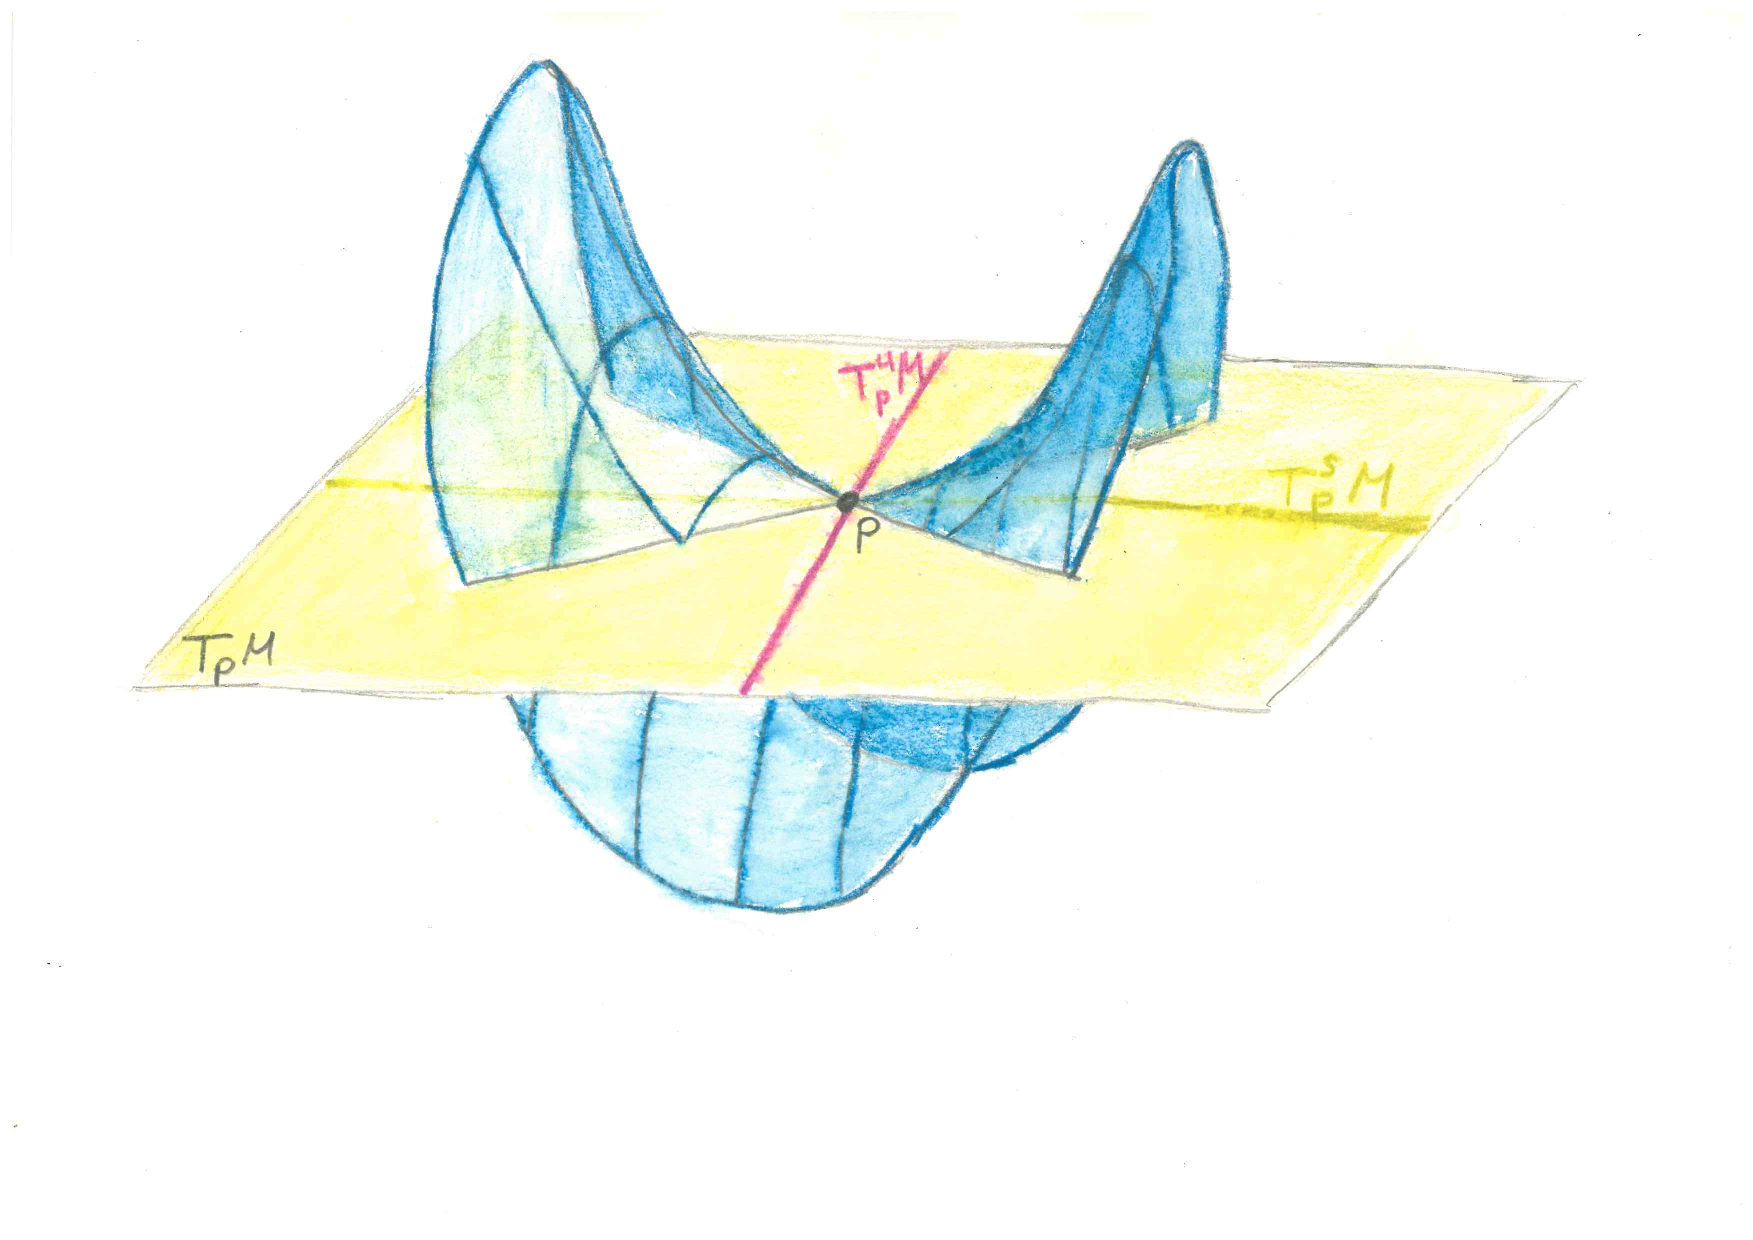
\includegraphics[width=0.9\textwidth]{Text/Pictures/Unstable Manifold/split tangend space.pdf}
	\caption{The splitting of the tangent space}
	\label{fig: The splitting of the tangent space}
\end{figure}

\begin{definition}[(un-)stable tangend space]
	For any map $\theta: T_p^sM\bigoplus T_p^uM\to T_pM$ we define the \textbf{stable set} of $\theta$ to be:
	\begin{equation*}
		W^s_r(\theta):=\{x\in T_pM| \forall n \geq 0, \theta^n(x) \text{ is defined and } \norm{\theta^n(x)} \leq r\}
	\end{equation*} The norm here is arbitrary as we are finite dimensional and therefore all norms are equivalent.
\end{definition}
\begin{remark}
	In the proof of the (un-)stable manifold theorem, we will map the stable set into such a stable set in the tangent space. So if we could control the structure of such a map, we would win. That is accomplished as the next theorem tells us that this set is the graph of a smooth function, and the projection of the graph onto the domain gives us then a differentiable structure.
\end{remark}


\begin{theorem}[local (un-)stable manifold theorem] \label{thm: local (un-)stable manifold theorem}
	We define:
	\begin{align*}
		T:=\diff \phi_t\big|_p,\quad T_s:=T\big|_{T_p^sM},\quad T_u:=T\big|_{T_p^uM}.
	\end{align*} Let $\lambda<1$ such that $\norm{T_s}<\lambda$ and $\norm{T_u^{-1}}<\lambda$, where $\norm{T}= \sup\{T(x)|\norm{x}\leq 1\}$ denotes the operator norm. Now for this setting there exists an $\varepsilon_{\lambda}$ depending only on $\lambda$, and there exists a $\delta>0$ for every $r>0$ which satisfy: For all $\theta:T_p^sM \times T_p^uM \to T_pM$ that satisfies $\theta-T$ is Lipschitz with Lipschitz constant
	\begin{equation*}
		\Lip(\theta-T)<\epsilon , \text{ and }\norm{\theta(0)}<\delta.
	\end{equation*}In this setting, 
	$W^s_r(\theta)$ is the graph of a Lipschitz function $g:T^s_pM\to T^u_pM$ with $ \text{Lip}(g)\leq 1$ and:
	\begin{enumerate}
		\item If $\theta$ is $C^k$ ($k$- times smooth differentiable), then so is $g$.
		\item If $\theta$ is smoothly differentiable ,$\theta(0)=0$ and $\diff \theta\big|_0=T$, then $g(0)=0$ and $\diff g |_0=0$. Hence, $T _pW^s_r(\theta)=T^s_pM$.
	\end{enumerate}
	A picture and application of this technical theorem is given in the proof of the global stable and unstable manifold theorem. 
\end{theorem}
\begin{proof}
	\todo{fehlt}
\end{proof}

\begin{figure}
	\centering
	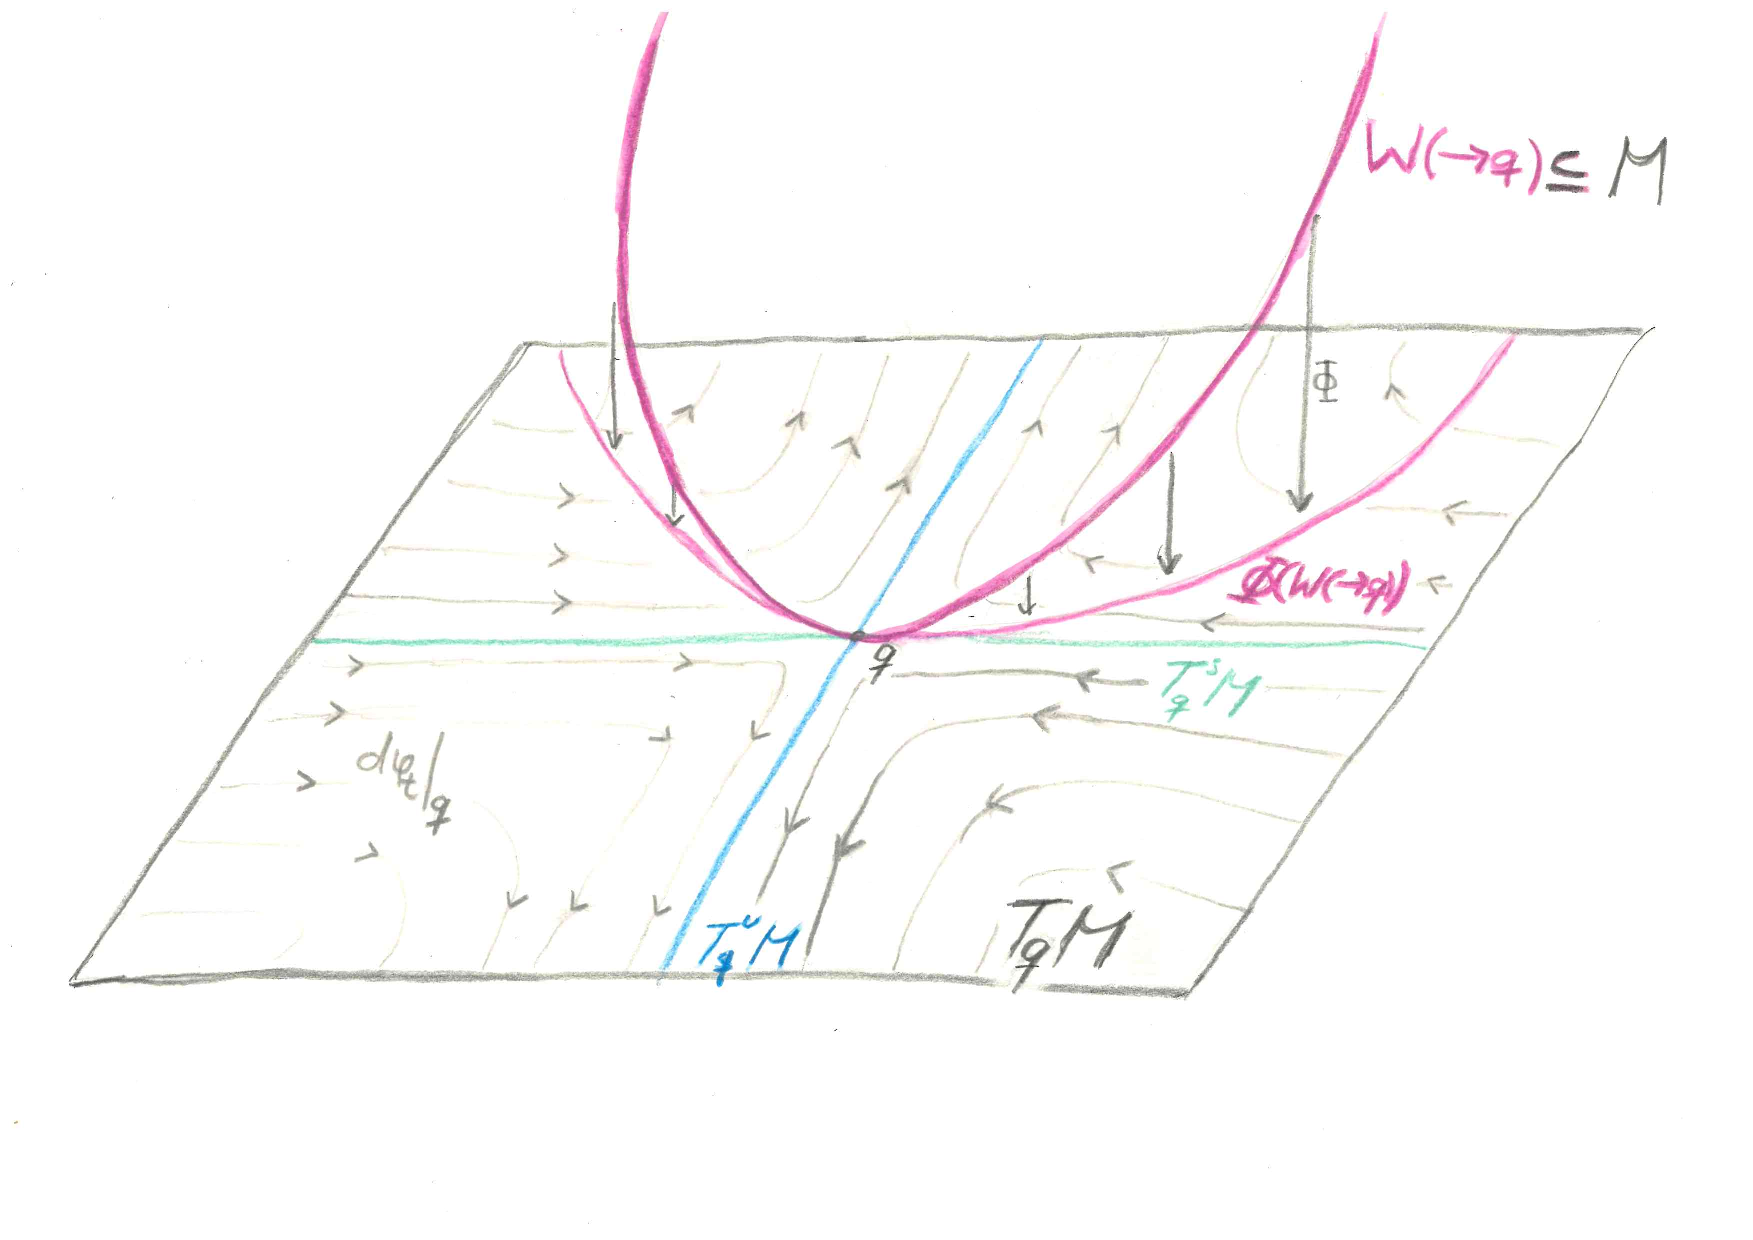
\includegraphics[width=0.9\textwidth]{Text/Pictures/Unstable Manifold/proof stable mfd thm.pdf}
	\caption{The proof of the (un-)stable manifold theorem}
	The Manifold is not shown in this image. One should imagen it looking like in figure \ref{fig: The splitting of the tangent space}. $p$ can be imagined to be the index sitting at the bottom of the hole of the tilted doughnut. 
	\label{fig: The proof of the (un-)stable manifold theorem}
\end{figure}

\begin{proof}[Proof of theorem \ref{thm: stable and unstable manifold theorem}] First we switch to the world of discrete dynamical systems and define $\phi:=\phi_1:M\to M$. The idea of the proof is to first find a chart for a small open subset of $W(\to p)=\{x\in M| \lim_{n\to \infty} \phi^n(x)=p\}$ arround $p$ and then define a global one. This is done by taking a small neighbourhood arround an arbetrary point $x\in W(\to p)$ and moving it via $\phi$ to the small neighbourhood of $p$.
	
	Let $U$ be a small neighborhood of $p \in M$ and  $\Psi:U \to T_pM$ be a centered coordinate chart (after identifying $\R^n $and $T_pM$ via $e_i \mapsto \partial q_i$). Now bx corollary \ref{cor: Tangendspace splits}, $T_pM$ splits into $T^s_pM\otimes T^u_pM$ with respect to $\diff \phi\big|_p$. If we inspect the image of $ W(\to p)\cap U$ under $\Phi$ we realise that it is a small pertubation of $T^s_pM$. This Situation can be seen in figure \ref{fig: The proof of the (un-)stable manifold theorem}. In fact, it is one that can be controlled using theorem \ref{thm: local (un-)stable manifold theorem}. For this we define $\theta:=\Psi\circ \phi \circ \Psi^{-1}:T_pM\to T_pM$. Now since $\theta$ is smooth we know that it is a lipschitz pertubation of $d\phi|_p$ and we can apply theorem \ref{thm: local (un-)stable manifold theorem} to conclude that there are indices $\epsilon$ and $r$ such that $W^s_r(\theta)$ is the graph of a smooth function. Notice that we might need to shrink the domain such that $\Lip(\theta-d\phi|_p)<\epsilon$. The next thing we want to do is to see that for a small neighbourhood $ U \ni p$
	\begin{equation}
		W^s_r(\theta)=\Psi(W(\to p)\cap U).
	\end{equation} This can be done by showing two inclusions: 
	\begin{itemize}
		\item $(\subset)$: for $x\in W^s_r(\theta)$ we can conclude that $\norm{\Psi \circ \phi^n \circ \Psi^{-1}}<r$ for all $n\in \N$. Now by Bolzano Weierstrass we know that $\lim_{n\to \infty}\Psi \circ \phi^n \circ \Psi^{-1}$ has at least one accumulation point. And since $p$ is hyperbolic by remark \ref{rem: critical points are hyperbolic fixpoints} we know this point is the origin and is unique. Therefor we conclude $\lim_{n\to \infty}\Psi \circ \phi^n \circ \Psi^{-1}=0$ which tells us that $\Psi^{-1}(x)\in W(\to p)\cap U$, where $U$ is a ball inside $\Psi^{-1}B_o(r)$.
		\item $(\supset)$ This direction is almost trivial. Let $y\in W(\to p)$ and $ x=\Psi(y)$. Since  $p$ is isolated we can choose $U$ small enough such that for all $y\in W(\to p)\cap U$ we have that $\theta^n(\Psi(y))<r $ for all $n\in \N$. For the last conclusion we might need to shrink $U$ further.
	\end{itemize}
	Now we know that $\Psi(W(\to p)\cap U)$ is the graph of a smooth function $g:T^s_pM\to T^u_pM$. Therefor, the projection $\pi(\Psi(W(\to p)\cap U))\subset T^s_pM$ gives us a chart. To get an Atlas for $W(\to p)$ we can define $U^n:=\phi^{-n}(U)$ for all $n$ to cover $W(\to p)$. This cover comes with charts defined by $(U^n,\pi \circ \Psi \circ \phi^n)$. For the sake of readability we define the charts $\chi^n:=\pi \circ \Psi \circ \phi^n$. Those charts are compatible since $\phi$ is a diffeomorphism. To conclude that we have a submanifold we need to check if the inclusion is an immersion. This however is clear by definition. 
	
	Finally, we want to prove that this submanifold is the image of a smooth embedding of $T^spM$. For this we define $B:= W(\to p)\cap U)$ and define $h:= \chi\circ \phi \circ \chi^{-1}$. Since similar Matrices have the same eigenvalues we can conclude that $\diff\chi|_0$ and $\diff \phi_p|_{T^s_pM}$ have the same eigenvalues.
	\color{red} Therefore, we can introduce an inner product such that the operator norm $\norm{dh_0}<1$. \color{black} Now let $\alpha\in \R$ and $B_0$ be a ball centred at $0$ such that $\norm{dh|_x} \leq \alpha$ for all $x\in B_0$. 
	Now this yields that $h|_{B_0}$ is a contraction, which we can extend to be a contraction $\tilde{h}:T^s_pM\to T^s_pM$. Now again similar as before we define a map $E^s:T^s_pM\to W(\to p)$ by first contracting, then going down and then expanding again. To be more precise, we define $E_n^s:\phi^{-n} \circ \chi^{-1} \tilde{h}^n$. 
	Finally, we define $E^s(x)=E^s_n(x)$ where $\tilde{h}^n(x)\in B_0$. Obviously, we need to check that this is well-defined: So assume that $n+1$ and $n$ work for $x$:
	\begin{align*}
		E^s_{n+1}(x)&=\phi^{-(n+1)}\circ \chi^{-1} \circ \tilde h^{n+1} \\
		&=\phi^{-(n+1)}\circ \chi^{-1} \circ h\circ \tilde{h}^{n} \\
		&=\phi^{-(n)}\circ \phi^{-1} \chi^{-1} \circ \underbrace{\chi \circ \phi \circ \chi^{-1}}_{h} \circ \tilde{h}^{n} \\
		&=\phi^{-n} \circ \chi^{-1} \circ \tilde{h}^{n}=E^s_n(x).
	\end{align*} To confirm that $E^s$ gives us an immersion onto $W(\to p)$ we first need to check for smoothness and bijectivity.By definition, we are smooth and by since all functions that compose to $E^s_n$, the latter is injective for all $n$. Now if $E^s_n(x)=E^s_m(y)$ with $m>n$, then $\tilde{h}^m(x)\in B_0$, since $\tilde{h}$ is a contraction and by the well definition we have $E^s_m(x)=E^s_m(y)$ which concludes to $x=y$, as the latter are injective for $m$. The surjectivity is also clear, as for all $x\in W(\to p)$ there is an $n$ such that $\phi^n(x)\in \chi^{-1}(B_0)$ and with that the point $\Tilde{h}^{-n}(\chi(\phi^n))$ does the job. So the last step is to verify that $\diff E^s|_x$ is injective. This follows from $\tilde{h}$ having an injective differential, since it is a contraction. Furthermore, $\chi^{-1}$ has an injective differential, as it is the inverse of a chart and $\phi$ has an injective differential, since $\diff \phi (x)=e^{-\frac{\partial}{\partial x}|_{\phi(x)}}$. The latter equality was shown in the proof of remark $\ref{rem: critical points are hyperbolic fixpoints}$. This concludes the proof for the stable set. For the unstable set we replace $f$ by $f^-1$. 
\end{proof}
\begin{cor}
	From the proof of the (un-)stable manifold theorem, we can deduce that $T_pW(\to p)=T^s_pM$.
\end{cor}
\begin{proof}
	For this we just use theorem \ref{thm: local (un-)stable manifold theorem} a bit more sophisticated. By the second statement of the theorem, we know that $T_pW^s_r(\theta)=T^s_p$. Notice that we actually talk about an equality here. But since $W^s_r(\theta)=\chi(W(\to p) \cap U)$ we know that $T_pW(\to p)=T^s_p$. 
\end{proof}

